%Capítulo 2

\section{Marco histórico y contextual}
    
    "La investigación en la UAG es una actividad que contribuye a dar coherencia a sus otras funciones sustantivas y tiene por objeto promover, alentar y apoyar a los esfuerzos que lleven a generar nuevo conocimiento en las áreas académicas que integran a la institución, contribuir a la solución de los problemas de la sociedad a nivel regional y nacional, mejorar la calidad del proceso enseñanza-aprendizaje para nuestros estudiantes, vinculando pertinentemente las actividades de investigación de los profesores en conformidad con la Misión, Valores y Fines de la Universidad Autónoma de Guadalajara.
    La investigación deberá ser realizada en todos los niveles educativos que ofrece la Institución y estará focalizada en proponer soluciones a los problemas planteados por los sectores productivos, social y de servicios tanto del sector público como del privado. Es por ello y siguiendo este propósito se pretende que con el Sistema de información de la Coordinación de Investigación y Desarrollo Tecnológico se tenga un registro de toda la investigación que se crean en nuestra Universidad, desde Tesis de cualquier Licenciatura o grado académico, hasta artículos, proyectos de intervención o bien cualquier tipo de investigación que sea relevante sin importar la etapa escolar en la que se esté."\cite{UAG}
    
    La página actual del sistema de investigadores de la Universidad Autónoma de Guadalajara, utiliza un diseño anticuado; antes del 2018, en el cual la mayoría de los elementos web son estáticos y, no se adaptan con fluidez a las resoluciones actuales en el año 2022, además, para incluir nuevas funcionalidades al sistema de investigadores se necesita modificar una gran cantidad de elementos web o, casi rediseñarlos, ya que la arquitectura monolítica utilizada en conjunto del patrón de diseño de Modelo-Vista-Controlador(MVC) no permite que se le agreguen nuevas funcionalidades de una manera sencilla.
    
    \begin{figure}[H]
        \centering
        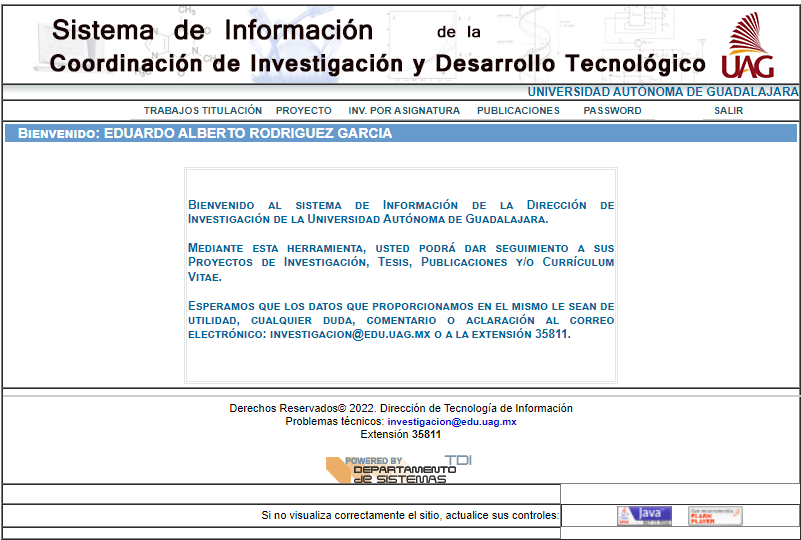
\includegraphics[width=\textwidth]{Propuesta_Plantilla_Tesis_LaTeX_UAG/imagenes/sistema_investigadores_actual.png}
        \caption{Actual sistema de investigadores.}
        \label{fig:homepage}
    \end{figure}
    
    La propuesta del equipo de trabajo liderado por la Doctora Lina María Aguilar Lobo consiste en volver a desarrollar el sistema de investigadores, pero con una nueva arquitectura y elementos que faciliten la implementación de nuevas funcionalidades. La arquitectura propuesta se compondrá de los siguientes elementos:
    
    \begin{itemize}
        \item Utilizar el patrón de diseño de Modelo-Vista-Controlador como base.
        \item Separar el desarrollo en dos partes: frontend y backend.
        \item Crear una base de datos relacional normalizada.
        \item Apoyarse de una arquitectura de micro servicios para proveer de información al frontend.
        \item Interfaz gráfica de usuario responsiva.
    \end{itemize}

\section{Marco referencial}
    
    La arquitectura actual usada en el sistema de investigadores es de tipo monolítico, la cual se centra en un solo proveedor o servidor para interactuar con el sistema de investigadores. Esto conlleva algunas desventajas:
    
    \begin{itemize}
        \item Si alguno de los módulos del sistema de investigadores falla, esto causará que todo el sistema falle.
        \item Acoplamiento estrecho.
        \item No es sencillo escalar el sistema de investigadores; dicho en otras palabras: agregar nuevas funcionalidades.
        \item Las tecnologías usadas en el sistema de investigadores se debe de usar en todo momento. Los cambios de tecnologías son costosos en términos de tiempo y de recursos.
    \end{itemize}
    
    La mayor diferencia entre una arquitectura monolítica y una de micro servicios se puede apreciar en los diagramas siguientes:
    
    \begin{figure}[H]
        \centering
        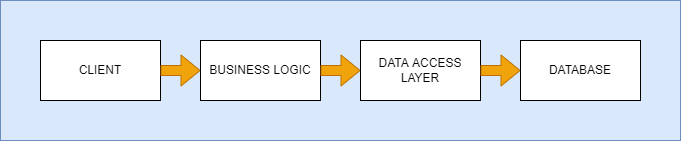
\includegraphics[width=\textwidth]{Propuesta_Plantilla_Tesis_LaTeX_UAG/imagenes/monolitico.png}
        \caption{Arquitectura monolítica.\cite{KryptonSolid}}
        \label{fig:monolitica}
    \end{figure}
    
    \begin{figure}[H]
        \centering
        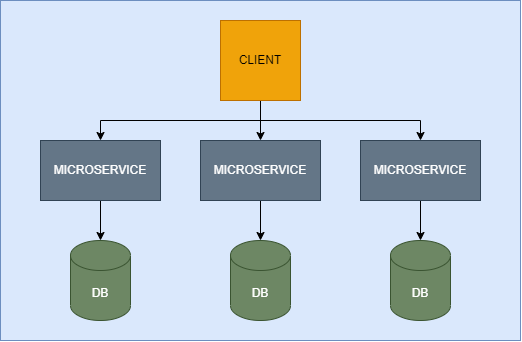
\includegraphics[width=\textwidth]{Propuesta_Plantilla_Tesis_LaTeX_UAG/imagenes/microservicios.png}
        \caption{Arquitectura basada en micro servicios.\cite{KryptonSolid}}
        \label{fig:micro-servicios}
    \end{figure}

\section{Marco Teórico}

    El nuevo sistema de investigadores que se implementa en este documento se basa en metodologías de trabajo ágiles, y así mismo de una arquitectura en el backend de micro servicios la cual traerá beneficios a la escalabilidad, acoplamiento, y gestión del sistema de investigadores.
    
    "La arquitectura de micro servicios divide los componentes del sistema en pequeños servicios autónomos que se pueden implementar y escalar de forma independiente."\cite{KryptonSolid}

    La arquitectura de micro servicios nos permite el separar cada funcionalidad en módulos específicos los cuales; al no estar estrechamente acoplados, no afectaran al sistema de investigadores si alguno presenta una falla. Además de que es más sencillo el proceso de debug y pruebas para estos módulos.

\section{Hipótesis}

    La necesidad de rehacer el sistema de investigadores yace en la habilidad de agregar nuevas funcionalidades para mejorar los procesos de los investigadores dentro de la UAG y, dado el conocimiento y habilidades de programación para backend se implementa la arquitectura de micro servicios para proveer el 100\% de la información dinámica requerida y almacenada en la base de datos a la parte del frontend la cual se encargarán otros alumnos de realizar.

\section{Definición de términos y conceptos básicos}

    \textbf{API}: Application Programming Interface.\cite{jacobson2012apis}

    \textbf{Arquitectura}: La arquitectura de software consiste en la estructura del sistema, combinado con las características arquitectónicas que el sistema debe soportar, las decisiones arquitectónicas, y finalmente los principios de diseño. \cite{richards2020fundamentals}
    
    \textbf{Arquitectura monolítica}:

    \textbf{Backend}: Hace referencia al desarrollo del lado del servidor. Se concentra en bases de datos, scripts, y arquitectura web. Contiene actividades detrás de escena que ocurren cuando se realizan acciones en el sitio web. \cite{Backend}
    
    \textbf{Base de datos}:
    
    \textbf{Debug}:
    
    \textbf{Desplegar}: 
    
    \textbf{Diseño web responsivo}: El diseño web responsivo es una configuración en la que el servidor siempre envía el mismo código HTML a todos los dispositivos y se usa CSS para modificar el procesamiento de la página en el dispositivo. Los algoritmos de Google deberían detectar automáticamente esta configuración si se permite que todos los usuarios-agentes del robot de Google rastreen la página y sus elementos (imágenes, CSS y JavaScript). \cite{GoogleResponsivo}
    
    \textbf{Endpoint}:
    
    \textbf{Frontend}:
    
    \textbf{HTTP}:
    
    \textbf{Micro servicios}: La arquitectura de micro servicios es un estilo que da estructura a una aplicación como una colección de servicios con las siguientes características\cite{richards2020fundamentals}:
    
    \begin{itemize}
        \item Altamente mantenibles.
        \item Se encuentran débilmente acoplados.
        \item Desplegables independientemente; no dependen de otros servicios.
        \item Organizados por capacidades del sistema
        \item Fáciles de probar.
        \item Pueden trabajar con diferentes tecnologías y lenguajes.
    \end{itemize}
    
    \textbf{MVC}: Modelo-Vista-Controlador
    
    \textbf{Módulo}:
    
    \textbf{Script}:
    
    \textbf{Servidor}:
    
    \textbf{UAG}: Universidad Autónoma de Guadalajara.
    
    \textbf{UML}: 
    
    \textbf{URI}: